\documentclass[a4paper,12pt]{article}
%%%%%%%%%%%%%%%%%%%%%%%%%%%%%%%%%%%%%%%%%%%%%%%%%%%%%%%%%%%%%%%%%%%%%%%%%%%%%%%%%%%%%%%%%%%%%%%%%%%%%%%%%%%%%%%%%%%%%%%%%%%%%%%%%%%%%%%%%%%%%%%%%%%%%%%%%%%%%%%%%%%%%%%%%%%%%%%%%%%%%%%%%%%%%%%%%%%%%%%%%%%%%%%%%%%%%%%%%%%%%%%%%%%%%%%%%%%%%%%%%%%%%%%%%%%%
\usepackage{eurosym}
\usepackage{vmargin}
\usepackage{amsmath}
\usepackage{graphics}
\usepackage{epsfig}
\usepackage{subfigure}
\usepackage{fancyhdr}

\setcounter{MaxMatrixCols}{10}
%TCIDATA{OutputFilter=LATEX.DLL}
%TCIDATA{Version=5.00.0.2570}
%TCIDATA{<META NAME="SaveForMode"CONTENT="1">}
%TCIDATA{LastRevised=Wednesday, February 23, 201113:24:34}
%TCIDATA{<META NAME="GraphicsSave" CONTENT="32">}
%TCIDATA{Language=American English}

\pagestyle{fancy}
\setmarginsrb{20mm}{0mm}{20mm}{25mm}{12mm}{11mm}{0mm}{11mm}
\lhead{MA4128} \rhead{Kevin O'Brien} \chead{Week 6} %\input{tcilatex}

\begin{document}

%%%%%%%%%%%%%%%%%%%%%%%%%%%%%%%%%%%%%%%%%%%%%%%%%%%%%%%%%%%%%%%%%%%%%%%%%%%%%%%%%%%%%%%%%%%%%%%%


\section{Likelihood Ratio Test}
\begin{itemize}
\item The likelihood ratio test is a test of the difference between -2LL for the full
model with predictors and ?2LL for initial chi-square in the null model.
\item When probability fails to reach the 5\% significance level, we retain the null hypothesis
that knowing the independent variables (predictors) has no increased effects (i.e. make no
difference) in predicting the dependent.
\end{itemize}



\section{Likelihood ratio test}
\begin{itemize}
\item The likelihood-ratio test test discussed above to assess model fit is also the recommended procedure to assess the contribution of individual "predictors" to a given model.

\item In the case of a single predictor model, one simply compares the deviance of the predictor model with that of the null model on a chi-square distribution with a single degree of freedom. If the predictor model has a significantly smaller deviance (c.f chi-square using the difference in degrees of freedom of the two models), then one can conclude that there is a significant association between the "predictor" and the outcome. 
\item Although some common statistical packages (e.g. SPSS) do provide likelihood ratio test statistics, without this computationally intensive test it would be more difficult to assess the contribution of individual predictors in the multiple logistic regression case. 
\item To assess the contribution of individual predictors one can enter the predictors hierarchically, comparing each new model with the previous to determine the contribution of each predictor.
\item There is considerable debate among statisticians regarding the appropriateness of so-called "stepwise" procedures. They do not preserve the nominal statistical properties and can be very misleading.
\end{itemize}

%%%%%%%%%%%%%%%%%%%%%%%%%%%%%%%%%%%%%%%%%%%%%%%%%%%%%%%%%%%%%%%%%%%%%%%%%%%%%%%%%%%%%%%%%%%%%%

\subsection{Log Likelihood}
A ``likelihood" is a probability, specifically the probability that the observed values of the dependent may be predicted from the observed values of the independents. 

Like any probability, the likelihood varies from 0 to 1. The log likelihood (LL) is its log and varies from 0 to minus infinity (it is negative because the log of any number less than 1 is negative). LL is calculated through iteration, using maximum likelihood estimation (MLE).


\subsection{Maximum Likelihood Estimation}
\begin{itemize}
\item Maximum likelihood estimation, MLE, is the method used to calculate the logit coefficients. This contrasts to the use of ordinary least squares (OLS) estimation of coefficients in regression. OLS seeks to minimize the sum of squared distances of the data points to the regression line. 
\item MLE seeks to maximize the log likelihood, LL, which reflects how likely it is (the odds) that the observed values of the dependent may be predicted from the observed values of the independents. (Equivalently MLE seeks to minimize the -2LL value.)

\item MLE is an iterative algorithm which starts with an initial arbitrary ``guesstimate" of what the logit coefficients should be, the MLE algorithm determines the direction and size change in the logit coefficients which will increase LL. 
\item After this initial function is estimated, the residuals are tested and a re-estimate is made with an improved function, and the process is repeated (usually about a half-dozen times) until convergence is reached (that is, until LL does not change significantly). There are several alternative convergence criteria.
\end{itemize}




\subsection{Log Likelihood}
A ``likelihood" is a probability, specifically the probability that the observed values of the dependent may be predicted from the observed values of the independents. 

Like any probability, the likelihood varies from 0 to 1. The log likelihood (LL) is its log and varies from 0 to minus infinity (it is negative because the log of any number less than 1 is negative). LL is calculated through iteration, using maximum likelihood estimation (MLE).


\subsection{Maximum Likelihood Estimation}
\begin{itemize}
	\item Maximum likelihood estimation, MLE, is the method used to calculate the logit coefficients. This contrasts to the use of ordinary least squares (OLS) estimation of coefficients in regression. OLS seeks to minimize the sum of squared distances of the data points to the regression line. 
	\item MLE seeks to maximize the log likelihood, LL, which reflects how likely it is (the odds) that the observed values of the dependent may be predicted from the observed values of the independents. (Equivalently MLE seeks to minimize the -2LL value.)
	
	\item MLE is an iterative algorithm which starts with an initial arbitrary ``guesstimate" of what the logit coefficients should be, the MLE algorithm determines the direction and size change in the logit coefficients which will increase LL. 
	\item After this initial function is estimated, the residuals are tested and a re-estimate is made with an improved function, and the process is repeated (usually about a half-dozen times) until convergence is reached (that is, until LL does not change significantly). There are several alternative convergence criteria.
\end{itemize}





\subsection{The Likelihood Ratio Test}
The likelihood ratio test to test this hypothesis is based on the likelihood
function. We can formally test to see whether inclusion of an explanatory variable in a model tells us
more about the outcome variable than a model that does not include that variable. Suppose
we have to evaluate two models. 
\begin{center}
	\begin{figure}[h!]
		% Requires \usepackage{graphicx}
		\includegraphics[scale=0.75]{LogWeek10D}\\
		\caption{Variables}
	\end{figure}
\end{center}
Here, Model 1 is said to be nested within Model 2 – all the explanatory variables in Model 1
(X1) are included in Model 2. We are interested in whether the additional explanatory
variable in Model 2 ($X_2$) is required, i.e. does the simpler model (Model 1) fit the data just as
well as the fuller model (Model 2). In other words, we test the null hypothesis that $\beta_2 = 0$
against the alternative hypothesis that $\beta_2 \neq 0$. 



\subsection{The Likelihood Ratio Test}
The likelihood ratio test to test this hypothesis is based on the likelihood
function. We can formally test to see whether inclusion of an explanatory variable in a model tells us
more about the outcome variable than a model that does not include that variable. Suppose
we have to evaluate two models. 
\begin{center}
	\begin{figure}[h!]
		% Requires \usepackage{graphicx}
		\includegraphics[scale=0.75]{LogWeek10D}\\
		\caption{Variables}
	\end{figure}
\end{center}
Here, Model 1 is said to be nested within Model 2 – all the explanatory variables in Model 1
(X1) are included in Model 2. We are interested in whether the additional explanatory
variable in Model 2 ($X_2$) is required, i.e. does the simpler model (Model 1) fit the data just as
well as the fuller model (Model 2). In other words, we test the null hypothesis that $\beta_2 = 0$
against the alternative hypothesis that $\beta_2 \neq 0$. 





\subsection{The Likelihood Ratio Test}
The likelihood ratio test to test this hypothesis is based on the likelihood
function. We can formally test to see whether inclusion of an explanatory variable in a model tells us
more about the outcome variable than a model that does not include that variable. Suppose
we have to evaluate two models. 
\begin{center}
	\begin{figure}[h!]
		% Requires \usepackage{graphicx}
		\includegraphics[scale=0.75]{LogWeek10D}\\
		\caption{Variables}
	\end{figure}
\end{center}
Here, Model 1 is said to be nested within Model 2 – all the explanatory variables in Model 1
(X1) are included in Model 2. We are interested in whether the additional explanatory
variable in Model 2 ($X_2$) is required, i.e. does the simpler model (Model 1) fit the data just as
well as the fuller model (Model 2). In other words, we test the null hypothesis that $\beta_2 = 0$
against the alternative hypothesis that $\beta_2 \neq 0$. 




\subsection{The Likelihood Ratio Test}
The likelihood ratio test to test this hypothesis is based on the likelihood
function. We can formally test to see whether inclusion of an explanatory variable in a model tells us
more about the outcome variable than a model that does not include that variable. Suppose
we have to evaluate two models. 
\begin{center}
	\begin{figure}[h!]
		% Requires \usepackage{graphicx}
		\includegraphics[scale=0.75]{LogWeek10D}\\
		\caption{Variables}
	\end{figure}
\end{center}
Here, Model 1 is said to be nested within Model 2 – all the explanatory variables in Model 1
(X1) are included in Model 2. We are interested in whether the additional explanatory
variable in Model 2 ($X_2$) is required, i.e. does the simpler model (Model 1) fit the data just as
well as the fuller model (Model 2). In other words, we test the null hypothesis that $\beta_2 = 0$
against the alternative hypothesis that $\beta_2 \neq 0$. 


	
	
\section{The Likelihood Ratio Test}
The likelihood ratio test to test this hypothesis is based on the likelihood
function. We can formally test to see whether inclusion of an explanatory variable in a model tells us
more about the outcome variable than a model that does not include that variable. Suppose
we have to evaluate two models. 

\begin{center}
\begin{figure}[h!]
% Requires \usepackage{graphicx}
\includegraphics[scale=0.6]{images/LogWeek10D}\\
\caption{Variables}
\end{figure}
\end{center}
Here, Model 1 is said to be nested within Model 2 – all the explanatory variables in Model 1
(X1) are included in Model 2. We are interested in whether the additional explanatory
variable in Model 2 ($X_2$) is required, i.e. does the simpler model (Model 1) fit the data just as
well as the fuller model (Model 2). In other words, we test the null hypothesis that $\beta_2 = 0$
against the alternative hypothesis that $\beta_2 \neq 0$. 

\end{document}
